\section{Abwägung des Einsatzes eines Informationsmanagements an der Hochschule Emden Leer}
Das Soll-Konzept analysiert die Ist-Situation um festzustellen, ob es generell einer Verbesserung des Informationsmanagements bedarf und wo diese anzusetzen sind oder ob noch kein Informationsmanagement besteht und aufgebaut werden muss. Dazu sind verschiedene Aspekte zu beleuchten. Neben der Anforderung des Marketings und neben den  technischen Neuerungen und Umsetzungen ist zu klären, wer die strategische und operative Führung übernehmen soll. 

Im klassischen Informationsmanagement ist dies die Aufgabe eines Chief Information Officers. Der Informationsmanager dient dabei als zentrale Schnittstelle zwischen technischen, organisatorischen und wirtschaftlichen Teilbereichen und dient dort als sogenannter Mittler und untersucht dafür die Informations- und Kommunikationstechniken in allen unterschiedlichen Bereichen um diese sinnvoll einzusetzen.\footnote{\cite[86]{krcmar_einfuhrung_2015}}

\begin{figure}[h!]
	\centering
	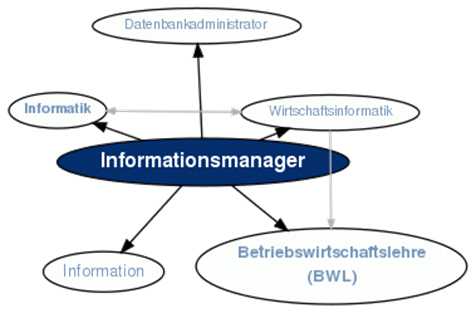
\includegraphics[width=10cm]{kapitel/gruppe3/bilder/definition_informationsmanager}
	\caption{Definition Informationsmanager}
	\label{fig_definition_informationsmanager}
\end{figure}

\subsection{Analyse des Ist-Zustandes}
Bezug nehmend auf die Abbildung \ref{fig_organigramm_HS} und der festgestellten Ist-Analyse ist festzuhalten, dass der Hochschule Emden kein Informationsmanagement im klassischen Sinne zugrunde liegt, sondern ein zentrales Informationssystem.

Es werden verschiedene Dienste und Möglichkeiten wie Moodle, Eduroam zur Verfügung gestellt und in Anspruch genommen.

Es gibt keine Verwaltung, sondern verschiedene Bereiche, die unterteilt sind in Arbeitsgruppen, Abteilungen sowie Rechenstelle und Pressestelle.

Weiterhin beinhaltet das Informationssystem verschiedene Prozesse zum Datenaustausch, bzw. Datenfluss und Backuptransfer  aus verschiedenen Systemen.\footnote{Ist-Situation \#8}

Die Nutzung des gegenwärtigen Informationssystems wird unterschiedlich stark genutzt oder ausgelastet.

Von den zentralen Einrichtungen nehmen das Hochschulrechenzentrum und die Bibliothek einen wichtigen Platz in der Hochschule ein. Das Hochschulrechenzentrum übernimmt derweil viele Aufgaben der Informationsverwaltung und Planung.

Doch nicht nur da werden Informationen gesammelt und  ausgewertet. Die Hochschule in Emden definiert eine ganze Reihe von Arbeitsgruppen, beispielsweise die Arbeitsgruppe Zahlen, Daten, Fakten, die Kennzahlen der Hochschule und der einzelnen Fachbereiche sammelt und diese auswertet.\footnote{Ist-Situation \#8}

Aktuell besteht keine Vernetzung verschiedener Intranetzsysteme zwischen verschiedenen Hochschulen.

\subsection{Analyse des zu erwartenden Soll-Zustandes}
Nach Betrachtung der Best-Practice Beispiele anderer Hochschulen, lässt sich erkennen, dass jede Hochschule und auch Universität den Umgang des Informationsmanagements anders angeht. So spielen verschiedene Faktoren eine Rolle, die an jeder Hochschule unterschiedlich ausgelegt sind.

Ein Vergleich der betrachteten Hochschulen mit der Hochschule Emden zeigt, dass Emden eine wesentlich kleinere Hochschule ist und somit andere Ansprüche sowie nicht so komplexe Strukturen besitzt, als beispielsweise die WWW Münster, die über 40.000 Studierende pflegt.

Trotz unterschiedlich integrierter Möglichkeiten zur Umsetzung des jeweiligen Informationsmanagements, gibt es doch Bereiche die gleich oder relativ ähnlich sind. So sind Bibliotheken, Gremien, Ausschüsse, ebenso wie Fachbereiche und auch das Präsidium Teil einer jeden Hochschule oder Universität.

Es ist zu schauen wo sich das Informationsmanagement ansetzen lässt um mehrere Bereiche und Bestandteile untereinander zu verbinden. Fakt ist, dass es in Emden bereits Arbeitsgruppen gibt, die bestimmte Informationen gewinnen und filtern. So wäre der Aufbau einer neuen Struktur eine Möglichkeit zur Verbesserung des Informationsaustausches.

\subsection{Soll-Möglichkeit}
\subsection{Zu erwartende Kosten}
\subsection{Prognose und zu erwartender Verlauf / Fazit}